\documentclass[journal,final,letterpaper,11pt]{IEEEtran}
\usepackage{multirow}
\usepackage{url}
\usepackage{cite}
\usepackage{graphicx}
\usepackage{algorithmic}
%\DeclareGraphicsExtensions{.png}
\begin{document}
\title{How to Cheat in Puzzles and Dragons}
\author{Amanda~Chow, Ted~Li, and~David~Zeng}
\markboth{CS 221 Project Proposal, Autumn 2015}{}
\maketitle

\section{Introduction}
\IEEEPARstart{P}{uzzles} and Dragons (PAD) is one of the most popular games on both  Android and iOS. It takes a unique approach to mobile gaming, combining aspects of both RPGs and puzzle games to create a game where you pick a team of monsters and level them up by battling evil monsters. During the battles, you play a matching puzzle game, which will be focus of our project.
\vspace*{-0.15in}
\subsection{Puzzle Gameplay}
\begin{figure}[h]
\vspace*{-0.1in}
\centering
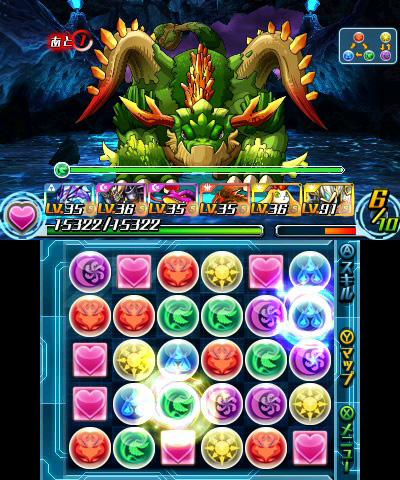
\includegraphics[scale=0.5]{pad.jpg}
\end{figure}
\vspace*{-0.1in}
The puzzles in the game present you with randomized puzzle board (shown above) with $5$ rows and $6$ columns. Each of these spaces contains one of six orbs: Fire, Water, Grass, Light, Dark, and Heart. To begin solving the puzzle, you select an orb and drag it. As you drag it through other orbs, the other orbs will swap locations with the orb you are dragging, effectively pushing the orbs in your path behind you. The goal of dragging the orb around is to position other orbs so that you form groups of orbs of the same color. Once you let go of your selected orb, or reach a $4$ second limit, your turn is completed. The game then finds groups of orbs of the same color and gives you a score based on the size of these groups and the number of groups.

\section{Gameplay Implementation}
Our project focuses on creating a AI designed for cheating on the puzzles. We decided to frame the PAD puzzle as the following problem: given a limited number of moves, what is the highest scoring path one can achieve on a random board? If our AI could find an optimal path to drag an orb around, then a human player could run the AI and follow its suggested path, and easily defeat the monsters in the dungeons.
\vspace*{-0.1in}
\subsection{Restrictions on the Game}
PAD allows the player unlimited time to think about the board, but only four seconds to drag around an orb. For a good player, this usually equates to dragging the orb around $40$ spaces after some initial thought to plan the path. Therefore, for our AI to fairly emulate what is possible for a human, it will also need to limit the number of moves it can execute on a turn to $40$. PAD also allows the player to drag an orb in all $8$ ordinal directions, but for most human players, diagonal dragging is very difficult to execute accurately, especially given the time limit and the small size of the mobile screen. Therefore, we chose to also limit our AI to only make moves in $4$ ordinal directions: up, down, left, right.
\vspace*{-0.1in}
\subsection{Evaluating the Board}
To properly evaluate the performance of our AI, we need a metric to evaluate the PAD puzzle board. Our evaluation metric performs the following algorithm.
\begin{enumerate}
\item Find all continuous groups of 3 or more orbs in single rows and columns.
\item Combine groups of the same color that either intersect or are adjacent.
\item Each group is given a score of $1 + \frac{1}{4}(\mbox{size} - 3)$. \item Sum the scores for each group.
\item Multiply by the sum by the combo multiplier, given by $1 + \frac{1}{4}(\mbox{\# of groups} - 1)$.
\end{enumerate}
The actual PAD game also takes into account orb types and how they interact with the offensive attributes of your team and the defenses of the actual monsters, but the pure mathematical score of the board is computed in an identical manner.

\section{Oracle}
It was difficult to find a guaranteed oracle for PAD, since there is no additional information beyond the puzzle board that is of any use. Even with a $40$ move limit and a ban on diagonal movements, there are far too many states to carry out an exhaustive search. We did discover a PAD web application that runs a search algorithm with greedy heuristics. Using our score metric, and a limit $40$ moves with no diagonal operations, the application averaged a score of roughly $15$, which corresponds to aligning $6$ groups of three orbs each.

\section{Baseline AI Implementation}
Our baseline AI implementation is based on a player making random moves. It performs the following algorithm.
\begin{algorithmic}[1]
\FOR{$i=1$ to $1000$}
  \STATE reset the board to original state
  \STATE pick a random orb to start
  \STATE $S_i :=$ score of board
  \STATE $P_i :=$ empty path
  \FOR{$j=1$ to $40$}
    \STATE drag the orb in a random direction
    \STATE $S :=$ score of board
    \IF{$S > S_i$}
      \STATE $S_i := S$
      \STATE $P_i :=$ path so far
    \ENDIF
  \ENDFOR
\ENDFOR
\RETURN $\max_{i}\{S_i\}$ and corresponding path $P_i$
\end{algorithmic}
We generated $100$ boards at random and ran our baseline algorithm on the boards and recorded its performance. The baseline achieved an average score of $7.38$ using an average path length of $25.31$. This roughly corresponds to the baseline algorithm being able to align $4$ groups of three orbs each.

\section{AI Improvements}
For the remainder of the quarter, our goal will be to improve upon our AI, utilizing various strategies from both human players and techniques from the course.
\vspace*{-0.15in}
\subsection{Human Strategies}
Because of the scoring mechanisms in this game, it is advantageous to find many groups of three rather than to look for larger groups, due to the combo multiplier that is applied in step $5$ of the board evaluation. Consequently, the predominant strategy for human players is to build their puzzle board up from the bottom, filling each row with two separate groups of three. From surveying multiple high level players, we found that they can typically make $6$ to $7$ groups of three per turn, resulting in scores that range from $13.5$ to $17.5$.
\vspace*{-0.15in}
\subsection{AI Strategies}
There are a variety of strategies we could try to improve our AI. The first would be to use reinforcement learning. We would need to collapse the state space of the PAD puzzle problem to something much smaller. One idea would be to base the state features around the notion of average distance between orbs of the same color. Grouping orbs involves bringing scatted orbs together, and so our reinforcement learning algorithm could locally reward moves that reduce distances between orbs of the same color.
\vspace*{-0.15in}
\subsection{Using Computer Vision}
In addition to improving the gameplay of our AI, we would also like to implement a computer vision component for the AI. This component would take in a screenshot of the game and use it to determine the board layout, allowing our AI to work directly off of a screenshot, which would be much more useful for dishonest players. Implementing such a vision component would require us to explore image segmentation techniques to detect the orbs.

\section{Related Work}
Here are some of the resources we plan to use to learn more about how to improve our AI.

\subsection{Reinforcement Learning}
In their paper, \textit{High-level Reinforcement Learning in Strategy Games}, Amato and Shani use Q-learning and Model-based Q-learning (Dyna-Q) to play a turn-based strategy game, Civilization IV. They do this by defining four state features - population difference, land difference, military power difference, and remaining land. Using these states, their AI applied the different reinforcement learning algorithms to find the best action to take each turn. In the Frederick versus Washington matchup, they found greatest success over their baseline of random policies with Dyna-Q, improving their win rate versus a fixed AI from $51\%$ to $62\%$.

\subsection{Computer Vision}
The notes in \cite{2} give a comprehensive comparison of various common segmentation algorithms, many of which are implemented in OpenCV. Understanding the pros and cons of these algorithms will be extremely useful in picking the right one for the computer vision component of the AI. For now, a mean-shift clustering approach might work well on the orbs, since each orb consists of similar shades of the same color.

\begin{thebibliography}{1}

\bibitem{1} Some shit on RL.
\bibitem{2} A Review of Computer Vision Segmentation Algorithms, \url{https://courses.cs.washington.edu/courses/cse576/12sp/notes/remote.pdf}


\end{thebibliography}

\end{document}


